\subsection{Introduction to traditional network traffic processing}
A \textit{network packet} is a basic unit of data transmitted over a network. It consists of a \textit{header}, which includes control information such as source and destination IP addresses, 
and a \textit{payload}, which carries the actual user data. 
Packets are routed independently through the network and reassembled at the destination. 
This structure allows efficient and reliable communication, even over complex or unreliable network paths.

Currently, packet processing works as follows: a packet arrives at the network card, which then
issues a system call (syscall) to the operating system for packet processing. The microprocessor
must save the currently executing instruction, perform a context switch, locate the appropriate
service routine in the interrupt vector table, and handle the packet processing. Once completed, it
must restore the saved instruction, perform another context switch, and return to processing the
interrupted program.

This system for operating peripherals was designed under the assumption that the peripherals
would not request interrupts continuously, which is not the case with network devices that need
to process large volumes of data split into small parts. 
This method requires the microprocessor to execute a significant
number of instructions not directly related to packet processing. 
Chase et al. \cite{gallatin1999trapeze} discovered \footnote{kap. 3.3 obr. 6} that if MTU is 1500 bytes, then interrupt handling accounts for 20\% - 25\% of receiver packet-processing overhead.
Another disadvantage of tradidtional packet processing is the inefficient handling of cache memory; the processing of the packets one by one in response to
interrupts leads to frequent cache misses in both cache \& inctruction caches.\footnote{kap. 4.2}\cite{cox2000profiling} 

%-----------------------------------------------------
\subsection{Vector Packet Processing: An Introduction}

%Co je VPP (Vector Packet Processing)
%Kdo ho vyvíjí (např. FD.io)
%Cíle a filosofie (výkon, modularita)
Vector Packet Processing (VPP) is a multi-platform network stack that operates at layers 2-4 of the ISO/OSI model and is developed by the FD.io project. 
It consists of a set of forwarding vertices arranged in an oriented graph and auxiliary software and provides out-of-the-box switch/router functionality.
Unlike traditional network stacks, which run in the kernel, VPP operates in user space.

In a traditional approach, packets are processed one by one. In contrast, VPP reads the largest available number of packets called vector from the network interface card (NIC) 
and processes the entire vector through a VPP node-graph one node at a time. Each node in this graph handles a specific part of the packet processing.
This approach reduces cache misses and spreads fixed overhead costs across multiple packets, lowering the average processing cost per packet. 
Additionally, it allows VPP to take advantage of multiple cores, enabling parallel processing, which significantly improves overall performance.

Vector Packet Processing (VPP) runs on common off-the-shelf hardware (COTS), ensuring its broad compatibility and flexibility for deployment. 
It supports various architectures such as x86, ARM, and Power, and can be deployed on both standard servers and embedded devices. 
The design of VPP is agnostic to hardware, kernel, and deployment platform, meaning it can operate across a wide range of systems, including bare metal servers, virtual machines (VMs), and containers. 
This approach allows VPP to be deployed on widely available infrastructure without the need for specialized hardware.\cite{fdio_what_is_vpp}

\subsection{Techniques used in VPP}
According to Linguaglossa et al.\cite{LINGUAGLOSSA} VPP uses theese kernel-bypass techniques:

\begin{itemize}
  \item \textbf{Lock-Free Multi-Threading (LFMT)}
is a programming technique that leverages modern multi-core CPUs to increase system performance. In network applications, parallelism is achieved by running multiple threads in the same time. 
Ideally, the more threads are used, the better the system performance but only up to a saturation point beyond which additional threads bring no gainns. 
However, to reach this ideal performance, traditional synchronization mechanisms such as mutexes and semaphores must be avoided, as they introduce delays due to thread contention. 
Instead, lock-free architectures have to be used, allowing threads to operate independently without blocking each other. 
In the context of VPP this approach is enabled by hardware features like multi-queue NICs, 
which allow each thread to handle a distinct subset of traffic, ensuring efficient and parallel processing.

  \item \textbf{I/O batching (IOB)}
is a key technique used in VPP. 
Instead of raising an interrupt for every incoming packet, the network interface card (NIC) collects multiple packets into a buffer and triggers an interrupt only when the buffer is full. 
This reduces the overhead caused by frequent context switching and interrupt handling. 
VPP typically uses poll-mode drivers, which collect packets in batches without relying on interrupts. 
Moreover, the batching technique is applied system-wide in VPP. This approach maximizes CPU efficiency, improves cache usage, and delivers stable, high-throughput performance even under heavy load.

  \item \textbf{Compute batching (CB)} 
is a technique that extends I/O batching to the processing phase itself. 
Instead of processing one packet at a time, network functions are designed to operate on entire batches of packets. 
This approach minimizes overhead from function calls (such as context switches and stack setup) and improves instruction cache efficiency. 
When a batch of packets enters a processing function, only the first packet might cause an instruction cache miss, while the rest benefit from already-warmed cache.
Additionally it is possible to take advatage of instruction-level parallelism.
  
  \item \textbf{Receive-Side Scaling (RSS)}
is a hardware-based technique used by modern NICs to distribute incoming packets across multiple RX queues. 
This enables parallel packet processing by allowing each queue to be handled by a separate thread, improving scalability and throughput. 
Packet assignment is typically done using a hash function over packet header fields (e.g., the 5-tuple). 

  \item \textbf{Zero-Copy (Z-C)} 
is a technique used to eliminate unnecessary memory copying during packet processing. 
Instead of copying incoming packets from the network interface card (NIC) to a separate buffer via system calls, 
the NIC writes packets directly into a pre-allocated memory region that is shared with the user-space application via Direct Memory Access (DMA). 
This allows the application to access packet data without invoking system calls or duplicating memory, significantly reducing CPU overhead. 

  \item \textbf {Cache Coherence and Locality (CC\&L)} are critical factors in the performance of modern software-based packet processing systems. 
In current COTS architectures, memory access has become a major bottleneck, which is mitigated by a multi-level cache hierarchy.
Minimizing cache misses and maintaining data locality during packet processing is essential for achieving high performance and low latency.

  \item \textbf {Low-Level Parallelism (LLP)} 
refers to the ability to exploit the internal micro-architecture of modern CPUs, including multi-stage pipelines, arithmetic-logical units (ALUs), and branch predictors that help maintain pipeline efficiency. 
Well-optimized code can keep these pipelines full and execute multiple instructions per clock cycle, increasing overall throughput. 
Performance can be further improved by giving hints to the compiler -- such as indicating the likely outcome of conditional branches -- to reduce pipeline stalls. 
Vectorized packet processing and specific coding practices can take full advantage of these hardware features and VPP was specifically designed to taky advantage of LLP.

\end{itemize}

\subsection{VPP Processing Graph and Graph nodes}
At the core of VPP (Vector Packet Processing) lies the Packet Processing Graph, a directed graph composed of relatively small, modular \& loosely coupled nodes. 
Each node is designed to perform a specific task and there are 3 types of them: \textit{process}, \textit{input} \& \textit{internal}. 
Process nodes do not participate in the packet forwarding graph; instead, they handle timers, events, and other background tasks within the VPP runtime.
Input nodes are used for input of data and internal nodes are used for vector processing. Internal nodes also serves as output nodes. 
When a vector of packets is prepared by input node, it is then pushed through the internal nodes. 
During processing, the vector may be split if the batch contains packets of different protocols or types, as they may need to follow different paths through the graph
When the original vector is completely processed, the process repeats.
Illustration of this Processing Graph is shown in fig. \ref{fig:processing-graph}.

\begin{figure}[!htbp]
    \centering
    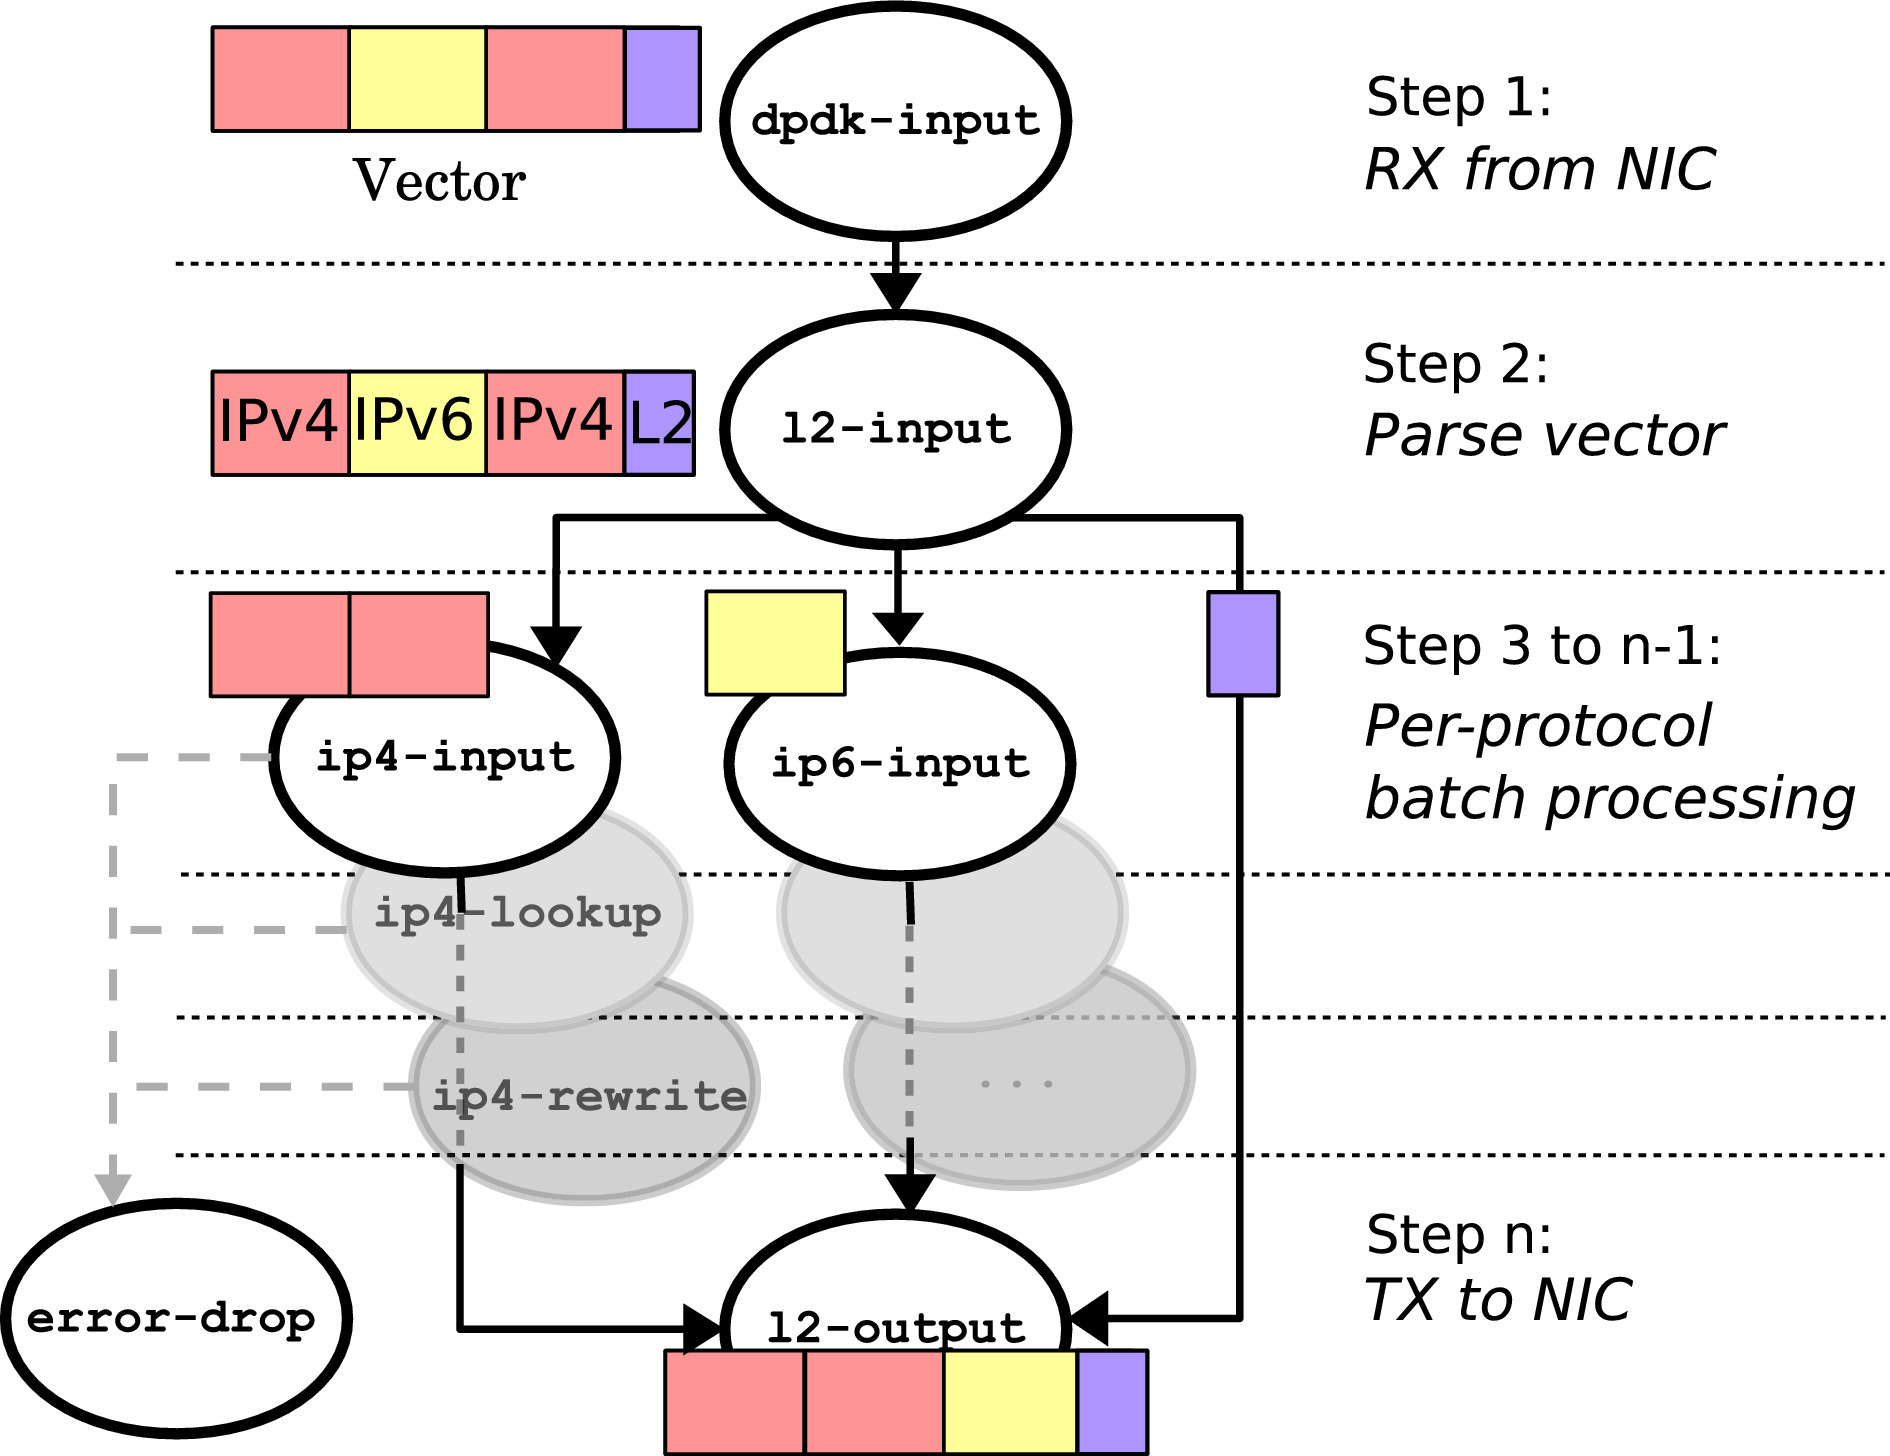
\includegraphics[width=0.7\linewidth]{images/processing-graph.jpg}
    \caption{Picture showing the VPP Processing Graph~\cite{LINGUAGLOSSA}}
    \label{fig:processing-graph}
\end{figure}

Thanks to VPP's modular design, the processing graph is highly customizable and extensible. 
New nodes -- referred to as plugins -- can be easily added to implement specific functionality or repleace existing ones. 
Plugins are shared libraries that are loaded during startup of VPP, and they are not dependent on the VPP source code, allowing them to be developed independently. 
Moreover, existing nodes can be rewired to modify the packet processing logic when necessary.\cite{LINGUAGLOSSA, DR:COMMAG-18, fdio_vpp_extensible_2021}




